%-----------------------------------------------------------------------------------------------
% 2020-NaaktgeborenC-PolyProc.tex - by C. Naaktgeboren
% License: CC-BY-NC-ND 4.0 - https://creativecommons.org/licenses/by-nc-nd/4.0/
%-----------------------------------------------------------------------------------------------
\documentclass[fleqn,11pt]{SelfArx}
%-----------------------------------------------------------------------------------------------
\usepackage[english]{babel}
\usepackage[squaren,cdot]{SIunits}
\usepackage{amsthm}
\usepackage{CormorantGaramond}
%-----------------------------------------------------------------------------------------------
\setlength{\abovecaptionskip}{4pt}
\setlength{\columnsep}{5.5mm}
\setlength{\columnseprule}{0.4pt}
\setlength{\fboxrule}{0.4pt} % Width of the border around the abstract
%-----------------------------------------------------------------------------------------------
\definecolor{color1}{RGB}{0,0,90} % Color of the article title and sections
\definecolor{color2}{RGB}{0,20,20} % Color of the boxes behind the abstract and headings
\definecolor{color3}{RGB}{0,0,192} % Color of the article title and sections
%-----------------------------------------------------------------------------------------------
\usepackage[hyperindex,breaklinks]{hyperref} % Required for hyperlinks
\hypersetup{%
    hidelinks,
    colorlinks,
    breaklinks=true,
    urlcolor=color3,
    citecolor=color1,
    linkcolor=color1,
    bookmarksopen=false,
    pdftitle={Title},
    pdfauthor={Author}
}
%-----------------------------------------------------------------------------------------------
\newtheorem{theorem}{Theorem}
\newtheorem{definition}{Definition}
\newtheorem{example}{Example}
%-----------------------------------------------------------------------------------------------
\makeatletter
\immediate\write18{datelog > \jobname.info} % site script: $(date -u '+%Y-%m-%d %Hh%Mm%Ss UTC')
\makeatother
%-----------------------------------------------------------------------------------------------
% Journal information
\JournalInfo{Preprints Server Name} % TODO: Update-me
\Archive{Compiled on \input{\jobname.info}}
% Article title
\PaperTitle{On Exact and Locally Polytropic Processes -- Requisites, Etymology, and Modeling}
\Authors{C.~Naaktgeboren\textsuperscript{1$\star$}}
\affiliation{\textsuperscript{1}\textit{Universidade Tecnológica Federal  do  Paraná  --  UTFPR,
Câmpus Guarapuava. Grupo de Pesquisa em Ciências Térmicas.}}
\affiliation{\textsuperscript{$\star$}\textbf{Corresponding  author}:
NaaktgeborenC$\cdot$PhD@gmail$\cdot$com}
\Keywords{Thermodynamics --- Polytropic  Processes  ---  Logical  Processes  ---  Etymology  ---
Modeling}
\newcommand{\keywordname}{Keywords}
\Remarks{%
    defines \emph{logical thermodynamic process} ---
    defines \emph{exact polytropic process} ---
    defines theoretical \emph{requisites} for exact polytropic process ---
    provides \emph{etymology} for the `polytropic' term ---
    presents a novel definition of \emph{locally polytropic process} ---
    proposes  \emph{locally  polytropic  processes}  as  \emph{building  blocks}   for   general
    engineering thermodynamics \emph{process modeling}.
}
\newcommand{\remarkname}{Remarks}
%-----------------------------------------------------------------------------------------------
\Abstract{Work in progress. Here goes the abstract...}
%-----------------------------------------------------------------------------------------------
\begin{document}
%-----------------------------------------------------------------------------------------------

\flushbottom

\maketitle

\tableofcontents

\thispagestyle{empty}

%-----------------------------------------------------------------------------------------------
\section*{License}

    \scriptsize\noindent%
    \begin{minipage}{\columnwidth}
        \centering\tt
        \includegraphics[height=6.0mm]{cc/by-nc-nd.pdf}\\[0.5\smallskipamount]
        {\scriptsize\url{https://creativecommons.org/licenses/by-nc-nd/4.0/}}
    \end{minipage}
    \normalsize

%-----------------------------------------------------------------------------------------------
\section{Introduction}

    Many equilibrium engineering thermodynamics processes  are  taken  to  follow  a  polytropic
    relationship  of  constant  $Pv^n$---in  which  $P$  is  the  system  pressure,  usually  in
    \kilo\pascal, $v$ is the system specific volume, usually  in  $\meter\cubed\!\per\kilogram$,
    and $n$ is the dimensionless polytropic  exponent~\cite{2013-CengelYA+BolesMA-AMGH}---which,
    for a ``1--2'' process, with initial and final end states labeled as ``1''  and  ``2'',  can
    also be written in terms of end states properties, as $P_1v_1^n = P_2v_2^n$.

    Some maintream thermodynamics textbooks introduce polytropic processes  in  the  context  of
    closed system boundary work, as a $P\!:\!P(v)$ relationship to plug  in  the  boundary  work
    integral,   which    contains    a    $P\,dv$    integrand~\cite{2013-CengelYA+BolesMA-AMGH,
    2002-MoranMJ+ShapiroHN-LTC, 1985-WylenG-Wiley}. In such texts, the  polytropic  relationship
    is frequently said to find support in measurents, while no specific  theoretical  derivation
    is presented at the point of introduction.

    On  the  other  hand,  other  texts~\cite{1986-JonesJB+HawkinsGA-Wiley,   2006-BejanA-Wiley,
    2015-KroosKA+PotterMC-Cengage} include derivations that lead to a polytropic process, or  at
    least to an isentropic version of it, in which the exponent $n$ has a determined value.

    Moreover, Bejan~\cite[p.~175]{2006-BejanA-Wiley} indicates that a constant  $Pv^n$  relation
    only holds \emph{locally} if the process is such that $n$ is a function of either $P$,  $v$,
    or both.

    A paper due to Christians~\cite{2012-ChristiansJ-IntJMechEngEduc} discusses the topic from a
    perspective  of  teaching  polytropic  processes  themselves,  placing   emphasis   on   the
    \emph{heat-to-work transfer ratio}---named by that author as ``energy transfer ratio''---and
    how its constancy not only yields, but constitutes a  pre-requisite  for  a  process  to  be
    polytropic, besides, naturally, the constancy of the caloric properties of the working  pure
    substance.

    This work proposes and develops the concepts of \emph{exact  polytropic}  and  \emph{locally
    polytropic} processes, and presents theory-derived \emph{requisites} for  a  process  to  be
    exactly polytropic. Moreover, an \emph{etymological} discussion is presented  in  connection
    to  the  usefulness  of  locally  polytropic  processes  as  discrete  building  blocks  for
    generalized equilibrium engineering thermodynamics process \emph{modeling}.

%-----------------------------------------------------------------------------------------------
\section{Exact and Locally Polytropic Processes}

    %---------------------------------------------------------------------------------------
    \subsection{Logical Processes}

    In equilibrium engineering thermodynamics, a \emph{process}---more properly  a  quasi-static
    or quasi-equilibrium one---is defined in terms of changes from a certain  equilibrium  state
    of a system to another~\cite{2013-CengelYA+BolesMA-AMGH}, with process \emph{path} being the
    (infinite) sequence of (quasi-)equilibrium states visited by the system during the  process.
    A process can be referred to by its path, with implicit or explicit end states.

    It is worth noting that no constraints are stated for the end states of  a  process  in  its
    definition.  This  allows  for  the  needed  flexibility  in  describing  the   variety   of
    transformations systems and control volumes can undergo in engineering thermodynamics.

    This lack of end state constraints in the definition of a process allows them to be splitted
    into multiple, successive `sub-processes' that still fit the definition  of  a  process,  as
    well as merged multiple successive ones together into `super-processes' that  also  fit  the
    definition of a process. This ability is extremely useful in grouping and splitting  systems
    and control volumes along with their underlying processes---a commom practice in engineering
    thermodynamics.

    Conversely, in order to  make  the  intended  distinction  between  proposed  ``exact''  and
    ``locally'' polytropic processes, additional constraints need to  be  made  to  process  end
    states. Thus, the following defines a  \emph{logical  thermodynamic  process},  which  is  a
    thermodynamic process with constrained end  states.  In  context,  i.e.,  in  thermodynamics
    texts, what's defined next can be simply called a ``logical process'':

    \begin{definition}[logical process]\label{def:logical.proc}
        A logical process is one in which its stated defining conditions, that determines all of
        the allowed interactions or property relations for  the  underlying  system  or  control
        volume, uniformly and continually apply to the  entirety  of  its  path  from---but  not
        earlier than---its initial state until---but not later than---its end state.
    \end{definition}

    Therefore,  for  a  simple  compressible  system---one  admitting   only   work   and   heat
    interactions---either stated heat and work interactions, or system property  specifications,
    or combinations of the two, define possible logical processes.

    Moreover, the stated defining conditions of a logical process can also carry  a  ``logical''
    qualifier, as to make it explicit they're being used in the definition of a logical process,
    as  in  the  ``logical  conditions,''  or  ``defining  logical   conditions''   expressions.
    Furthermore, the conditions themselves can carry the ``logical''  qualifier,  for  the  same
    purpose.

    \begin{example}\label{ex:ideal.Diesel}
        The   well-known   air-standard   ideal   Diesel    power    cycle,    illustrated    on
        Figure~\ref{fig:cycle.Diesel}, with ``intake'' state (of lowest temperature and pressure
        and maximum specific volume) labeled as ``1'', can be divided in  different  ways  using
        only logical processes. One such division is:  (i)~``logical  isentropic  compression'',
        ($\Delta s\!=\!0 \therefore Q\!=\!0$, $W\!\!<\!0$), (ii)~``logical  isobaric  heating'',
        ($Q\!>\!0$,  $\Delta  P\!=\!0   \therefore   W\!\!>\!0$),   (iii)~``logical   isentropic
        expansion'', ($\Delta s\!=\!0  \therefore  Q\!=\!0$,  $W\!\!>\!0$),  and  (iv)~``logical
        isochoric  cooling'',  ($Q\!<\!0$,  $\Delta  v\!=\!0   \therefore   W\!\!=\!0$),   which
        correspond, respectively, to the ``1--2'', ``2--3'', ``3--4'', and  ``4--1''  processes,
        i.e., to the canonical  processes  for  this  cycle,  excluding  sub-processes  thereof.
        Another possible division is: (a)~``logical isentropic compression'',  ($\Delta  s\!=\!0
        \therefore   Q\!=\!0$,   $W\!\!<\!0$),   (b)~``logical   no-heat-removal    expansion'',
        ($Q\!\geqslant\!0$, $W\!\!>\!0$), and  (c)~``logical  isochoric  cooling'',  ($Q\!<\!0$,
        $\Delta v\!=\!0 \therefore W\!\!=\!0$), which correspond, respectively, to the ``1--2'',
        ``2--4'' (through ``3''), and ``4--1'' processes, excluding sub-processes thereof, since
        these encompass the farthermost end states that uniformly and  continually  embrace  the
        stated defining logical conditions (a), (b), and (c).
    \end{example}

    \begin{figure}[ht]
        \centering
        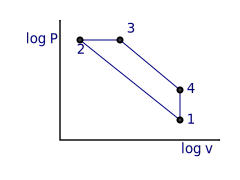
\includegraphics[width=40mm]{fig/idealDieselExample.pdf}
        \caption{Air-standard ideal Diesel cycle in  logarithmic  $P\times  v$  coordinates,  in
            support for the Example~\ref{ex:ideal.Diesel}.}
        \label{fig:cycle.Diesel}
    \end{figure}

    %---------------------------------------------------------------------------------------
    \subsection{Exact Polytropic Processes}

    \begin{definition}[exact polytropic process]\label{def:exact.poly.proc}
        An exact polytropic process is a logical process for which there is a unique  polytropic
        relation $Pv^n = \mbox{const.}$, with a unique, constant exponent $n$, that  holds  true
        for all states in the process path; or an isochoric logical process.
    \end{definition}

    It is worth noting that isochoric processes are equivalent to polytropic processes  with  $n
    \to \pm\infty$ between stated end states. Definition~\ref{def:exact.poly.proc} accounts  for
    the isochoric process non-unique polytropic exponent by explicitly including it as  a  valid
    exact polytropic process. The following is an inclusive theorem:

    \begin{theorem}[Matching definition]\label{theo:matching.def}
        Any logical process defined by  a  unique,  constant-polytropic  exponent  relation  and
        non-identical end states is an exact polytropic process.
    \end{theorem}

    \begin{proof}
        Such logical process definition statement fulfills the definition criteria for an  exact
        polytropic process, and therefore is, by definition, an exact polytropic process.  Since
        such logical process definition prohibits the end states to be identical, the uniqueness
        of the polytropic relation is  guaranteed,  for  if  end  states  ``1''  and  ``2''  are
        identical, then $P_1v_1^n = P_2v_2^n$ for any exponent $n$ since $P_1 = P_2$ and $v_1  =
        v_2$; otherwise, only the defining $n$ would cause the relation to  hold  true  for  all
        states in the process path.
    \end{proof}

    The matching definition theorem, or Theorem~\ref{theo:matching.def}, is instrumental in
    recognizing (and proposing) valid exact polytropic processes. The following is an exclusive
    theorem:

    \begin{theorem}[Same end states]\label{theo:same.end.states}
        No process, logical or otherwise, for which the end states are identical, is an exact
        polytropic process.
    \end{theorem}

    \begin{proof}
        If a process is not a logical one, it can't  be  an  exact  polytropic  process  by  its
        definition. This leaves one only with identical  end  states  logical  processes.  Since
        polytropic relationships $Pv^n = \mbox{const.}$ are monotonical, the only  way  its  end
        states are identical is in the case of a no-process. From  the  proof  of  the  matching
        definition Theorem~\ref{theo:matching.def},  the  unicity  of  such  polytropic  process
        exponent   cannot   be   established,    thus    proving    the    same    end    states
        Theorem~\ref{theo:same.end.states}.
    \end{proof}

    The same end states  theorem,  or  Theorem~\ref{theo:same.end.states},  is  instrumental  in
    ruling out any process for which a condition holds true for  a  single  state  as  an  exact
    polytropic  process,  as  is  the  case  of  recasting  a  constant  $Pv^n$  relation   with
    \emph{continuously varying} $n$ as an (infinite) set of constant polytropic exponent logical
    processes. From the same end states theorem one concludes that \emph{no} sub-process of such
    a process is an exact polytropic process.

    \begin{theorem}[Cycle]\label{theo:cycle}
        No cycle is an exact polytropic process.
    \end{theorem}

    \begin{proof}
        Since the defining feature of a cycle is same end states,  the  validity  of  the  cycle
        theorem, Theorem~\ref{theo:cycle}, follows directly from the validity of  the  same  end
        states theorem, Theorem~\ref{theo:same.end.states}.
    \end{proof}

    %---------------------------------------------------------------------------------------
    \subsection{Locally Polytropic Processes}

    For a polytropic process, one has: %
    %
    \begin{align}
        Pv^n & = c_1 = \text{const.}        & \rightharpoondown\\
        \log(Pv^n) & = \log(c_1) \equiv c_2 & \rightharpoondown\\
        \log P + n\log v & = c_2            & \rightharpoondown\\
        \log P & = -n\log v + c_2. \label{eq:affine}
    \end{align}

    Equation~(\ref{eq:affine}) is an affine relationship between $\log P$ and $\log v$---a  line
    segment within the polytropic process end states---in  which  the  polytropic  exponent  $n$
    figures as the negative of the line segment slope.

    Figure~\ref{fig:cycle.Diesel} is drawn in $\log P \times \log v$  coordinates,  and  depicts
    one line segment between each adjacent labeled state  pair  ``1--2'',  ``2--3'',  etc.  This
    means  all  roman-numbered  logical  process  in  Example~\ref{ex:ideal.Diesel}  are   exact
    polytropic processes, since (i)~they are logical processes that (ii)~can be represented by a
    unique polytropic relation with constant $n$.

    Figure~\ref{fig:non.exact} illustrates a process that plots as a curved segment in  $\log  P
    \times \log v$ coordinates. Basic derivative knowledge allows us to think of such process as
    one with a continuously variable slope in double logarithmic $P\times v$ coordinates.

    \begin{figure}[ht]
        \centering
        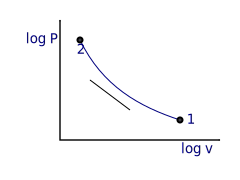
\includegraphics[width=40mm]{fig/nonExactPolytropic.pdf}
        \caption{A process displaying a curve in logarithmic $P\times v$ coordinates.}
        \label{fig:non.exact}
    \end{figure}

    Attempting to represent the process as a set of straight line segments would  result  in  an
    infinite set of segments of vanishing length---hence, same end states. The same  end  states
    theorem allows us to conclude that \emph{nowhere} along such a process one  finds  an  exact
    polytropic process.

    If, however, one allows for approximation, as is commom practice in engineering, the  curved
    process can be represented by an increasing but  finite  number  of  line  segments  with  a
    decreasing amount of deviation. The beginning of such a process is depicted on
    Figure~\ref{fig:approx}.

    \begin{figure}[ht]
        \centering
        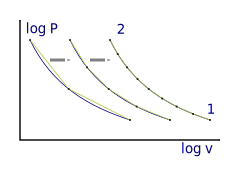
\includegraphics[width=40mm]{fig/approximations.pdf}
        \caption{Successive approximations to the curved process by means of 2, 4,  and  8  line
            segments in logarithmic $P\times v$ coordinates.}
        \label{fig:approx}
    \end{figure}

%-----------------------------------------------------------------------------------------------
\section*{Acknowledgments}

    This research received no specific grant from any funding agency in the public, private,  or
    not-for-profit sectors.

%-----------------------------------------------------------------------------------------------

\bibliographystyle{plain}
\bibliography{bibfile}

%-----------------------------------------------------------------------------------------------
\end{document}
%-----------------------------------------------------------------------------------------------
